\documentclass{article}[12pt]

% useful packages
\usepackage{fullpage}
\usepackage{amsmath,amssymb,amsthm,amsfonts}
\usepackage{graphicx}
\usepackage{enumerate}
\usepackage{algorithm,algorithmic}
\usepackage{xcolor}
\usepackage{bbm}
\usepackage{url}
\usepackage{caption,subcaption}

% theorem type environments
\newtheorem{thm}{Theorem}
\newtheorem{prop}{Proposition}
\newtheorem{lemma}{Lemma}
\newtheorem{cor}{Corollary}
\newtheorem{defn}{Definition}
\newtheorem{assump}{Assumption}
\newtheorem{example}{Example}
\newtheorem{conjecture}{Conjecture}

% frequently used symbols
\newcommand{\bE}{\mathbb{E}}
\newcommand{\bP}{\mathbb{P}}
\newcommand{\bQ}{\mathbb{Q}}
\newcommand{\bR}{\mathbb{R}}
\newcommand{\bS}{\mathbb{S}}
\newcommand{\bN}{\mathbb{N}}
\newcommand{\bZ}{\mathbb{Z}}
\newcommand{\sC}{{\mathcal C}} 
\newcommand{\sD}{{\mathcal D}} 
\newcommand{\sE}{{\mathcal E}} 
\newcommand{\sF}{{\mathcal F}} 
\newcommand{\sL}{{\mathcal L}} 
\newcommand{\sH}{{\mathcal H}} 
\newcommand{\sN}{{\mathcal N}} 
\newcommand{\sO}{{\mathcal O}} 
\newcommand{\sP}{{\mathcal P}} 
\newcommand{\sR}{{\mathcal R}} 
\newcommand{\sS}{{\mathcal S}}
\newcommand{\sU}{{\mathcal U}} 
\newcommand{\sX}{{\mathcal X}} 
\newcommand{\sY}{{\mathcal Y}} 
\newcommand{\sZ}{{\mathcal Z}}

% operators
\newcommand{\sign}{\mathop{\mathrm{sign}}}
\newcommand{\supp}{\mathop{\mathrm{supp}}} % support
\newcommand{\argmin}{\operatornamewithlimits{arg\ min}}
\newcommand{\argmax}{\operatornamewithlimits{arg\ max}}
\newcommand{\dist}{\operatorname{dist}}
\newcommand{\tr}{\text{tr}}
\newcommand{\vecop}{\text{vec}}
\newcommand{\st}{\operatorname{s.t.}}
\newcommand{\cut}{\setminus}
\newcommand{\ra}{\rightarrow}
\newcommand{\ind}[1]{\mathbbm{1}\left\{#1\right\}} 
\newcommand{\given}{\ | \ }

% grouping operators
\newcommand{\brac}[1]{\left[#1\right]}
\newcommand{\set}[1]{\left\{#1\right\}}
\newcommand{\abs}[1]{\left\lvert #1 \right\rvert}
\newcommand{\paren}[1]{\left(#1\right)}
\newcommand{\norm}[1]{\left\|#1\right\|}
\newcommand{\ip}[2]{\left\langle #1,#2 \right\rangle}

% code commands
\newcommand{\matlab}{\textsc{Matlab }}
\newcommand{\algname}[1]{\textnormal{\textsc{#1}}}

% header command
\newcommand{\homework}[4]{
    \pagestyle{myheadings}
    \thispagestyle{plain}
    \newpage
    \setcounter{page}{1}
    \setlength{\headsep}{10mm}
    \noindent
    \begin{center}
    \framebox{
        \vbox{\vspace{2mm}
            \hbox to 6.28in { {\bf STAT 672: Statistical Learning II
            \hfill Winter 2020} }
        \vspace{4mm}
        \hbox to 6.28in { {\Large \hfill Homework #1 \hfill} }
        \vspace{2mm}
        \hbox to 6.28in { \Large \hfill Due: #2 \hfill }
        \vspace{2mm}
        \hbox to 6.28in { {\it Student Name: #3} \hfill {\it Professor Name: #4}}
        \vspace{2mm}}
   }
   \end{center}
   \markboth{Homework #1}{Homework #1}
   \vspace*{4mm}
}

\begin{document}
\homework{3}{February 12th, 2020}{Ethan Lew}{Bruno Jedynak}

\section{Kernel approximation}
Kernel methods typically require to compute the kernel $(p,p)$ matrix 
\begin{equation}
K_{ij}=K(x_i,x_j)
\end{equation}
for $x_1,\ldots,x_p \in \mathcal{X}$. 
If $p$ is too large, say $p\geq 10^4$, this is prohibitive. Instead, one might want to find a low rank approximation. Here is one way to do it: 
\begin{enumerate}
\item choose $n < p$ elements $z_1,\ldots,z_n \in \mathcal{X}$, with $n$ not too large, say $n \leq 10^3$. One way is to choose them is at random.  
\item Notate as usual $H$ the RKHS with kernel $K$. 
\item Consider $V \subset H$, the subspace of $H$ spanned by the functions $K(.,z_i)$, for $1 \leq i \leq n$. 
\item Approximate for any $x,y \in \mathcal{X}$,
\begin{equation}
K(x,y) \sim \langle \pi_V(K(.,x),\pi_V(K(.,y) \rangle_H 
\end{equation}
where $\pi_V$ denote the orthogonal projection onto $V$. 
\end{enumerate}

Assume that $K_n$, the $(n,n)$ matrix with elements $[K_n]_{ij}=K(z_i,z_j)$ is positive definite. Notate $K(x,Z)=(K(x,z_1),\ldots,K(x,z_n))^T$. 
\begin{enumerate}
\item Show that 
\begin{equation}
	\pi_V (K(.,x)) = \sum_{i=1}^n \alpha_i(x)K(.,x_i) \mbox{ with } \alpha_i(x)=K_n^{-1}K(x,Z)
\end{equation}

\textbf{Solution:} Recall that the orthogonal projection $\pi_V(f)$ can be found by the optimization problem,
\begin{equation}
	\pi_V(f) = \operatorname*{argmin}_{g \in V} || g - f ||_{\mathcal H}^2.
\end{equation}
From the problem statement, it is clear that $g$ can be represented as,
\begin{equation}
	V = \operatorname{span}(\{K(.,z_i): 1 \le i \le n\}) \implies g = \sum^{n}_{i=1} \alpha_i K(., z_i), \quad \alpha_1,...,\alpha_n \in \mathbb R. 
\end{equation}
Return to the original statement, $\pi_V(K(.,x))$. The expression can be minimized by choosing a correct series of coefficients, $\alpha'$, from the objective $J(\alpha)$,
\begin{equation}
	\alpha' = \operatorname*{argmin}_{\alpha \in \mathbb R^n} J(\alpha) = \operatorname*{argmin}_{\alpha \in \mathbb R^n} \left|\left|K(., x) - \sum^{n}_{i=1} \alpha_i K(., z_i) \right|\right|_{\mathcal H}^2.
\end{equation}
Manipulate the expression,
\begin{equation}
	\begin{aligned}
		\left|\left|K(., x) - \sum^{n}_{i=1} \alpha_i K(., z_i) \right|\right|_{\mathcal H}^2 &= K(x,x) - 2 \sum^{n}_{i=1} \alpha_i K(x, z_i) + \sum^{n}_{i=1} \sum^{n}_{l=1} \alpha_i \alpha_l K(z_i, z_l)\\
												      &= K(x,x) - 2 K(x, Z)^T \alpha + \alpha^T K_n \alpha \\ 
	\end{aligned}
\end{equation}
Find the gradient of the LHS,
\begin{equation}
	\nabla_\alpha J(\alpha) = -2 K(x, Z) + 2 K_n \alpha. 
\end{equation}
Setting to zero, and from the convex nature of the problem, it is clear that 
\begin{equation} \label{eq:alpha_opt}
	\alpha' = K_n^{-1} K(x, Z).
\end{equation}

\item show that 
\begin{equation}
 \langle \pi_V(K(.,x),\pi_V(K(.,y) \rangle_H = K(x,Z)^T K_n^{-1} K(y,Z)
 \end{equation}
 
 Note that this method provides the approximation 
 \begin{equation}
K(x,y) \sim \phi(x)^T \phi(y) 
\end{equation}  
 where $\phi(.)=K_n^{-\frac{1}{2}}K(.,Z)$ is a vector in $\mathbb{R}^n$.

 \textbf{Solution:} Use the results from Equation \ref{eq:alpha_opt} and apply the bilinearity property,
 \begin{equation}
	 \begin{aligned}
		 \langle \pi_V(K(.,x),\pi_V(K(.,y) \rangle_H &= \langle K(x, Z)^T K_n^{-1} K(., Z), K(y, Z)^T K_n^{-1} K(., Z) \rangle_{\mathcal H}\\
							     &= \sum^{n}_{i=1} \sum^{n}_{j=1} \left[ K(x, Z)^T K_n^{-1} \right]_i \left[ K(y, Z) K_n^{-1} \right]_j K(x_i, x_j) \\
							     &= \sum^{n}_{i=1} \sum^{n}_{j=1} \left[ K(y, Z)^T K_n^{-1} \right]_i^T K(x_i, x_j) \left[ K(x, Z) K_n^{-1} \right]_j \\
							     &= K(y, Z)^T K_n^{-1} K_n K_n^{-1} K(x, Z) \\
							     &= K(y, Z)^T K_n^{-1} K(x, Z) \\
	 \end{aligned}
 \end{equation}
 

\item Show that the RKHS over $\mathcal{X}$ with kernel $G(x,y)=\phi(x)^T\phi(y)$ is made of the functions $f_w(.)=w^T\phi(.)$, where $w \in \mathbb{R}^d$.

	\textbf{Solution:} To demonstrate the RKHS, it is necessary to find a Hilbert space and a kernel $K$ satisfying the properties,
	\begin{enumerate}[(i)]
		\item \[
				\langle K(., x), f_w \rangle_{\mathcal H} = f_w(x)
		\]
		\item \[
				\mathcal H = \operatorname{span}(\{K(., x): x \in \mathcal X\}) 
		\] 
	\end{enumerate}
Note that the second condition is satisfied trivially as
\begin{equation}
	g \in V \implies g = \sum^{n}_{i=1} \alpha_i K(., x_i), \alpha \in \mathbb R^n. 
\end{equation}
Now, for the reproducing property,
\begin{equation}
	\begin{aligned}
		\langle K(., x), f_w \rangle_{\mathcal H} &= \langle K(., x), w^T K_n^{-1/2} K(., Z) \rangle_{\mathcal H}\\
							  &= \sum^{n}_{i=1} \left[ w^T K_n^{-1/2} \right]_i \langle K(., x), k(., z_i) \rangle_{\mathcal H} \\
									     &= \sum^{n}_{i=1} \left[w^T K_n^{-1/2} \right]_i K(x, z_i)\\
									     &= w^T K_n^{-1/2} K(x, Z) \\
									     &= f_w(x).
	\end{aligned}
\end{equation}



 \end{enumerate}
 \section{Kernel K-means}
 
 In this exercise I walk you through the spectral algorithm for finding an approximate solution of kernel k-means. 
 
 Let $x_1,\ldots,x_n$ be $n$ points in a set $\mathcal{X}$. We have seen in class that the relaxation of the kernel k-means problem consists in solving 
 \begin{equation}
 \label{eq:kmeans}
 \max_{S,S^T S=I_k} \mbox{trace}\left(S^T K S\right)
 \end{equation}
 where $S$ is an $(n,k)$ matrix, with $n>k$ and $K$ is a psd matrix with at least $k$ non-zero e-values. 
 \begin{enumerate}
 \item Let us write $S=(S_1,\ldots,S_k)$, where $S_j$ are vectors of length $n$. 
 Verify that 
 \begin{equation}
 \mbox{trace}S^TKS = \sum_{j=1}^k S_j^T K S_j
 \end{equation}

 \textbf{Solution:} Given a matrix $A \in \mathbb R^{n \times n}$, its trace can be calculated with
 \begin{equation}
	 \operatorname{trace}(A) = \sum^{n}_{i=1} [A]_{ii}. 
 \end{equation}
 The $ij$ element of the $n\times n$ matrix $S^T KS$ is,
 \begin{equation}
	 [S^T K S]_{ij} = S_i^T K S_j.
 \end{equation}
 So,
 \begin{equation}
	 {S^T K S}= \sum^{n}_{j=1} S_j^T K S_j. 
 \end{equation}

\item  Consider now the problem 
 \begin{equation}
 \label{eq:2}
 \max_{S,S_j^TS_j=1,j=1\ldots k} \mbox{trace}\left(S^TKS\right)
 \end{equation}
 Using Lagrange multipliers $\lambda=(\lambda_1,\ldots,\lambda_k)^T$, solving this problem is equivalent to solving 
 \begin{equation}
 max_{S,\lambda} J(S,\lambda) 
 \end{equation}
 with 
 \begin{equation}
 J(S,\lambda) =  \sum_{j=1}^k S_j^T K S_j - \sum_{j=1}^k \lambda_j S_j^TS_j
 \end{equation}
  Compute the gradients with respect to $S_j$ of $J(S,\lambda)$ for $j=1\ldots k$ and show that these gradients vanish when $S_1,\ldots,S_k$ are e-vectors of $K$ with e-values $\lambda_1,\ldots,\lambda_k$. 

\textbf{Solution: } Take the gradient of $J$ with respect to $S_j$, 
	 \begin{equation}
	\nabla_{S_j} J(S, \lambda) = 2K S_j -  2 \lambda_j S_j.  \\
\end{equation}
It is desired to find the critical points of $\nabla_{S_j}J$. Accordingly,
\begin{equation}
	\begin{aligned}
		\nabla_{S_j} J(S, \lambda) &= 2K S_j - 2 \lambda_j S_j = 0 \\
								    &\implies 2 K S_j = 2 \lambda_j S_j \\
								    &\implies K S_j = \lambda_j S_j\\
	\end{aligned}
\end{equation}
This implies, then, that $S_j$ is parallel to one of the eigenvectors of $K$. 

%Suppose that $\lambda_j$ is chosen such that it doesn't equal the $j^\text{th}$ largest eigenvalue of $K$. Such that,
%	 \begin{equation}
%		 K=U \Lambda U^T, \quad UU^T=I, [\Lambda]_{ij} \begin{cases} \tau_i, \quad i=j \\ 0 \quad i \ne j  \end{cases}.
%	 \end{equation}
%	 Now, given the eigendecomposition of $K=U\Lambda U^T$, consider $S_j = \mu u_j$, where $\mu \in \mathbb R$ and $u_j$ is the $j^{\text{th}}$ eigenvector of $U$,
%\begin{equation}
%\begin{aligned}
%	\sum^{k}_{j=1} 2 K S_j - \sum^{k}_{j=1} 2 \lambda_j S_j &= \sum^{k}_{j=1} 2 U \Lambda U^T S_j - \sum^{k}_{j=1} 2 \lambda_j S_j \\
%								&= \sum^{k}_{j=1} 2 \tau_j \mu  U e_j - \sum^{k}_{j=1} 2 \lambda_j u_j \\
%								&= \sum^{k}_{j=1} 2 u_j \mu \tau_j - \sum^{k}_{j=1} 2 u_j \lambda_j \\
%\end{aligned}
%\end{equation}
%Thus, when $\mu \tau_j = \lambda_j$,
%\begin{equation}
%	\left. \nabla_{S_j }J(S, \lambda)\right|_{S=\mu u_j, \lambda_j = \mu_j \tau_j }= 0.
%\end{equation}

 \item Choose these e-vectors to be orthogonal and with norm 1. Compute then $J(S,\lambda)$ and show that $\lambda_1,\ldots,\lambda_K$ have to be chosen to be the largest $k$ eigenvalues of $K$.

%	 \textbf{Solution:} As the norm is $\mu=1$, substituting from above,
%	 \begin{equation}
%	 	S_j = \lambda_j u_j, \quad \lambda_j = \tau_j,
%	 \end{equation} 
%	 where $\lambda_j, u_j$ are the $j^\text{th}$ largest eigenvalue and associated eigenvector respectively. Recognizing that $K$ can be decomposed into a form that explicitly contains its eigencomponents in an ordered fashion simplified the analysis required. 

	 \textbf{Solution: } For $J(S, \lambda)$,
	 \begin{equation}
		 \begin{aligned}
			 J(S, \lambda) &= \sum^{k}_{j=1} u_j^T K u_j - \sum^{k}_{j=1} \lambda_j u_j^T u_j   \\
								  &= \sum^{k}_{j=1} \lambda_j u_j^T u_j - \sum^{k}_{j=1} \lambda_j u_j^T u_j  \\  
								  &= 0 .  
		 \end{aligned}
	 \end{equation}
	 Make the substitution, $S_j = u_j$, where $u_j$ is some normalized eigenvector associated with an eigenvalue,
	 \begin{equation}
		 \begin{aligned}
			 \operatorname{trace}(S^T K S) &= \sum^{k}_{j=1} u_j^T K u_j  \\
								  &= \sum^{k}_{j=1} \lambda_j u_j^T u_j \\  
								  &= \sum^{k}_{j=1} \lambda_j .  
		 \end{aligned}
	 \end{equation}
	 It is clear, then, that this sum is maximized by choosing the $k$ largest eigenvalues. Thus, $S_j$ is the eigenvector associated with the $j^{\text{th}}$ largest eigenvalue, being the value chosen for $\lambda_j$.


 \item Argue that you have solved (\ref{eq:kmeans}).

	 \textbf{Solution: } The critical points of the Lagrange multiplier find points where the objective function and constraints have gradients parallel to one another, differing by a factor of $\lambda$. When this is not the case, either the objective input or constraint input can be changed to result in a greater objective function. So, this approach was valid to find the maximum of Equation \ref{eq:kmeans}. 

	 Intuitively, the process is similar to performing kernel PCA before clustering. The clustering now occurs in a space where observations are represented with an uncorrelated basis in the RKHS, structuring the data in a way that is potentially simpler to cluster.
 
 \item This provides a recipe for solving kernel k-means: 
 \begin{enumerate}
 \item compute $S=(S_1,\ldots,S_k)$, the matrix of the first $k$ e-vectors of the matrix $K$. This is equivalent to mapping each point $x_i$ to the vector of $\mathbb{R}^k$, 
 \begin{equation}
 \phi(x_i)=(S_{1i},\ldots,S_{ki})
 \end{equation}
 \item Solve the clustering problem using a classical clustering algorithm, that is k-means or the Estimation Maximization algorithm (E.M.) fpr the data $\phi(x_1),\ldots,\phi(x_n)$
 \end{enumerate}
 Apply this to the data in file \mbox{kkm1.csv} for $k=2$. Use a package of your choice for the clustering algorithm. 
 
 \textbf{Solution:} See Figures \ref{fig:orig} and \ref{fig:gauss}.

 \item Show some results with a different kernel;

	 \textbf{Solution:} See Figure \ref{fig:poly}.
\end{enumerate}  

\begin{figure}
	\centering
	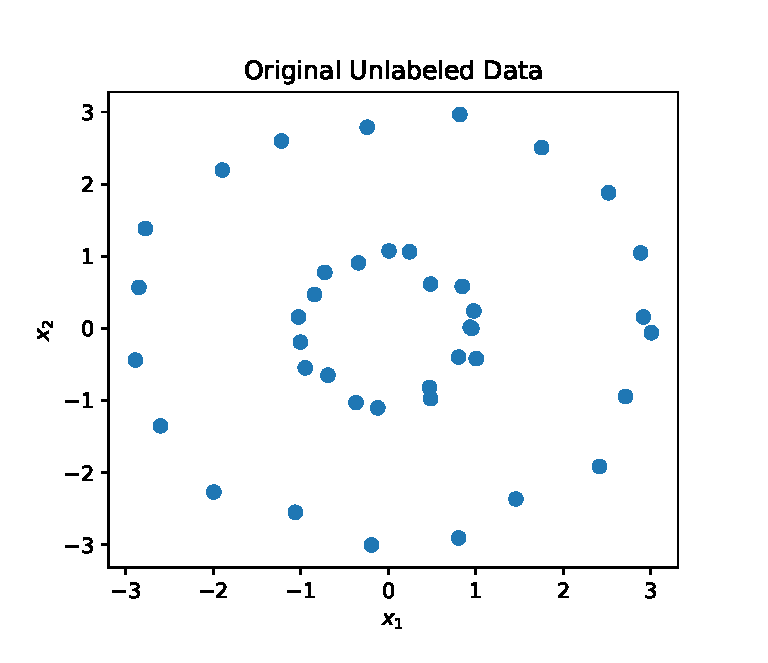
\includegraphics[width=0.4\linewidth]{img/original_data.eps}
	\caption{Data Supplied for This Problem}%
	\label{fig:orig}
\end{figure}

\begin{figure}
	\centering
	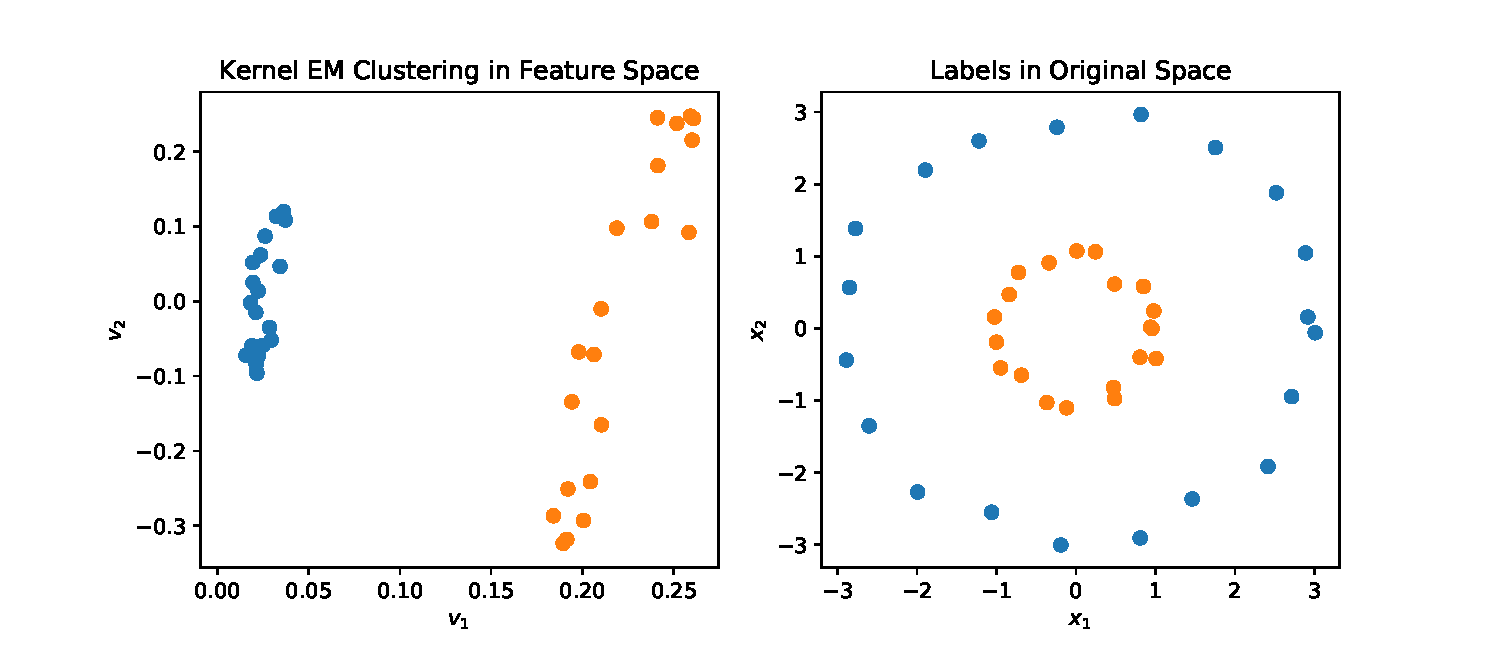
\includegraphics[width=0.8\linewidth]{./img/gaussian_1.eps}
	\caption{Kernel $k$-Means with Gaussian Kernel $\tau=1$}%
	\label{fig:gauss}
\end{figure}

\begin{figure}
	\centering
	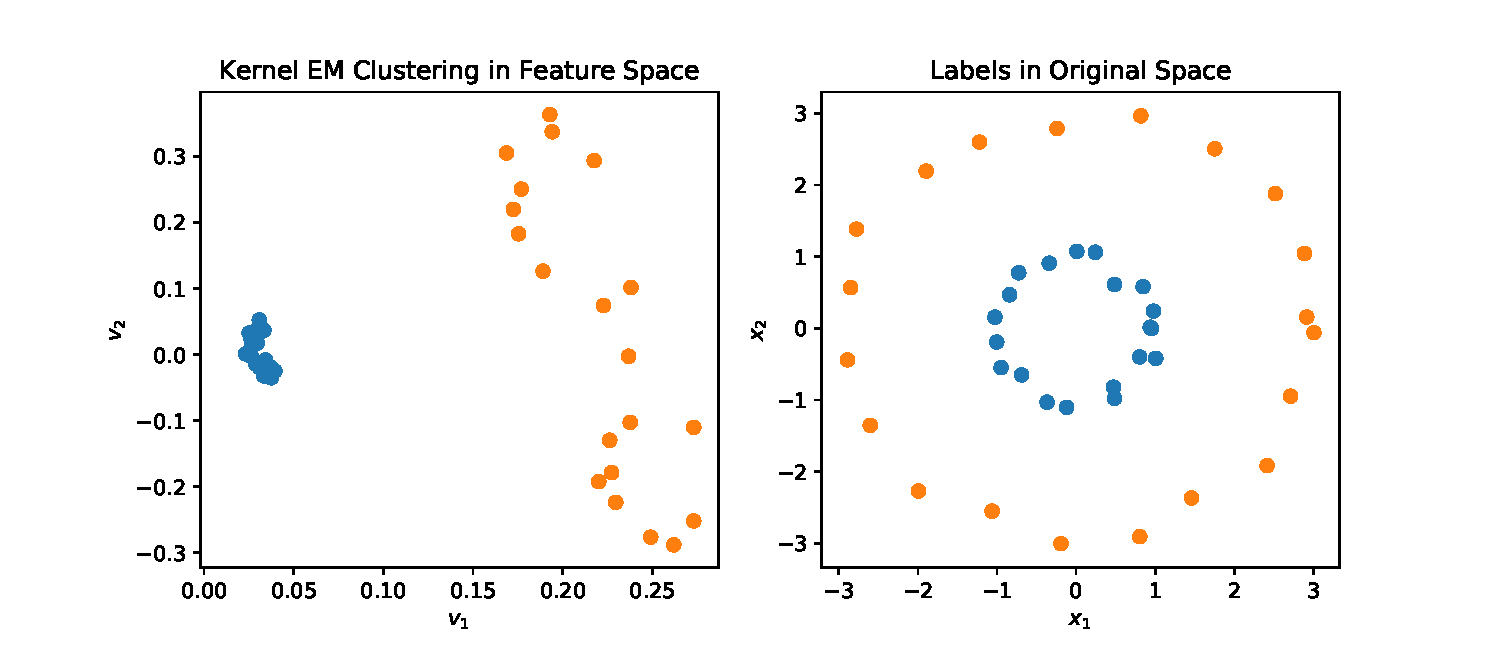
\includegraphics[width=0.8\linewidth]{./img/polynomial_2.eps}
	\caption{Kernel $k$-Means with Polynomial Kernel $d=2$}%
	\label{fig:poly}
\end{figure}
%\begin{figure}
%	\centering 
%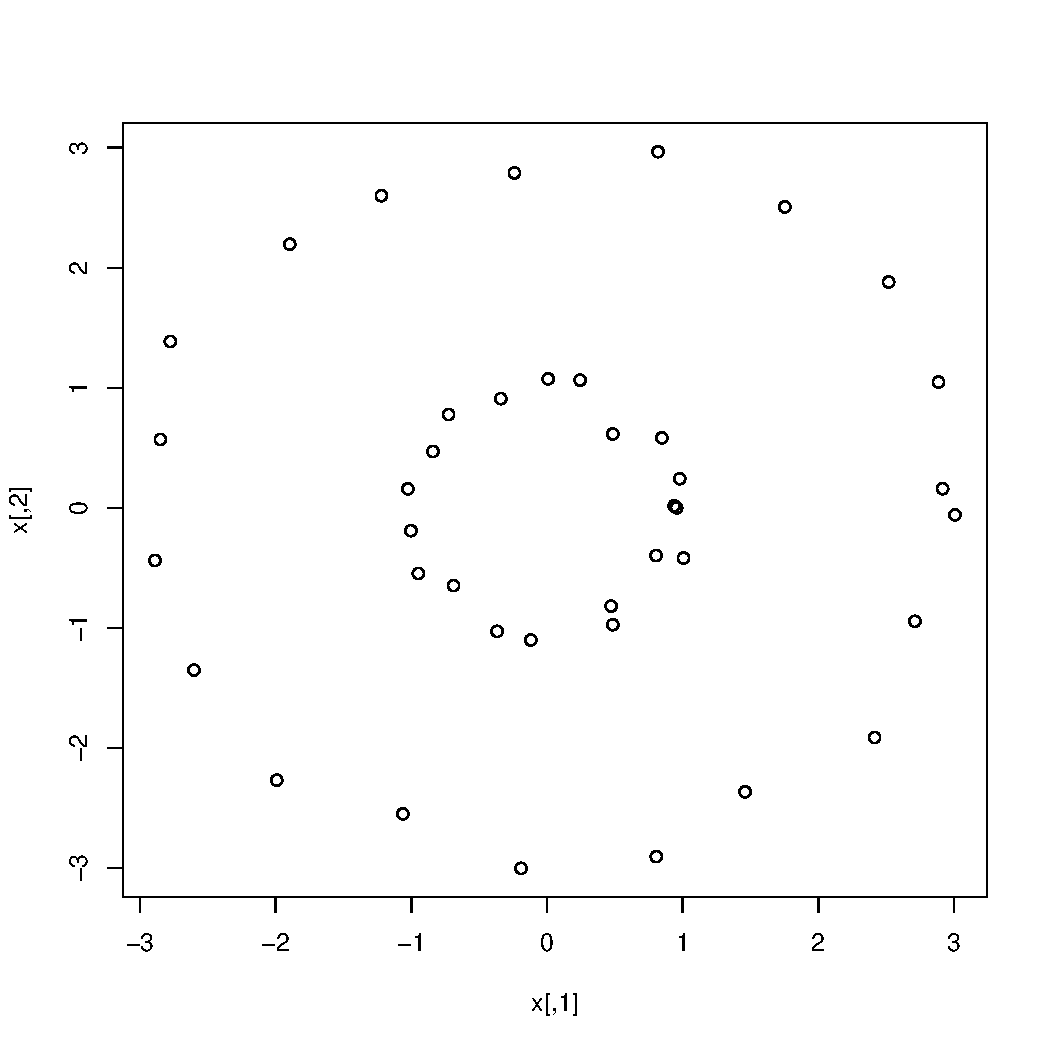
\includegraphics[width=0.3\textwidth]{img/data_for_kkm1.pdf}
%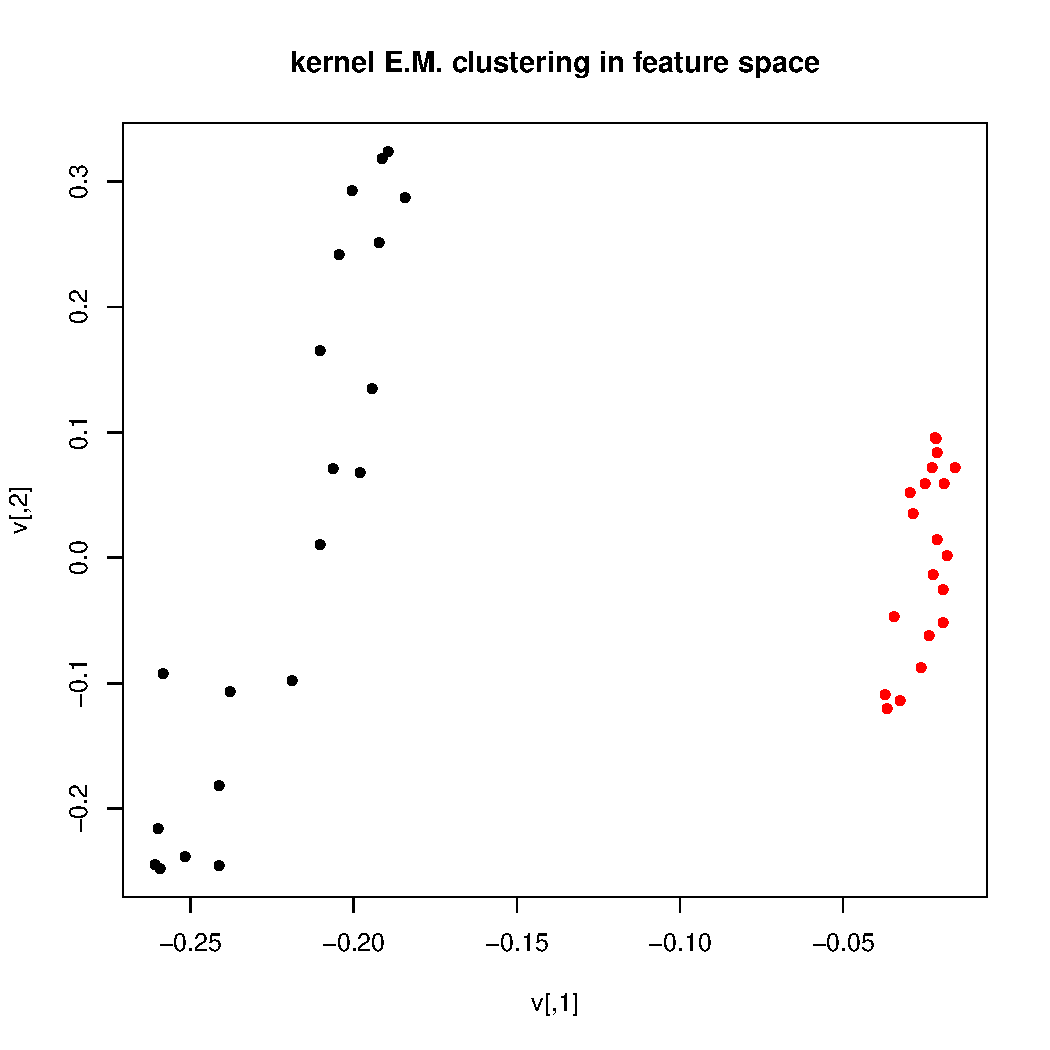
\includegraphics[width=0.3\textwidth]{img/kkmeans_feat.pdf}
%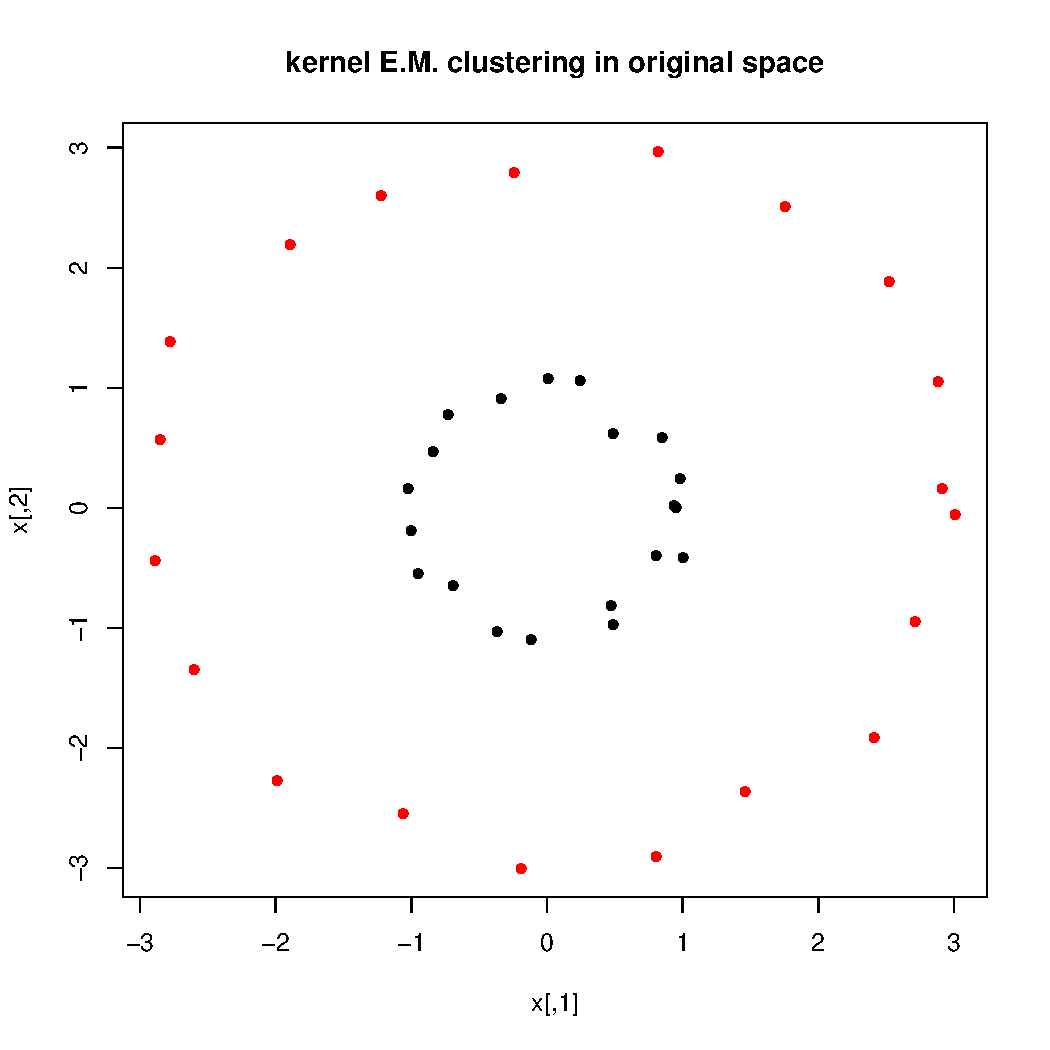
\includegraphics[width=0.3\textwidth]{img/kkmeans_orig.pdf}
%\caption{Kernel k-means}
%\end{figure}

\end{document}
